%
% ch03 解释器
% 讲解Lisp解释器的组成部分。
%

{
    \let\centering\raggedright
    \chapter{解释器结构}
    \label{ch:interp structure}
}    \thispagestyle{hubu@thesis}


本章节讨论一般Lisp解释器的结构,相关的技术以及EdenApple这个解释器实现的具体结构。EdenApple的VM与Compiler主要参考R. Kent Dybvig的Three implementation models for scheme\cite{dybvig87timpl}中的Heap-based model。语义上的细节主要参考scheme语言规范r6rs\cite{r6rs}。

解释器的工作原理在\textit{Essentials of Programming Language\cite{friedman2001eopl}}中有很好的描述,本论文的实现亦有沿用其中的思路。

EdenApple的基本结构如图\ref{fig:interp structure}所示:

\begin{figure}[h]
\begin{center}
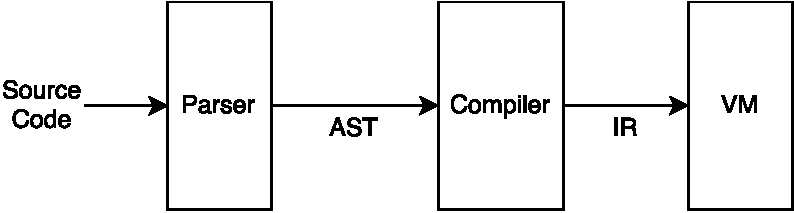
\includegraphics[width=\textwidth]{interpreter}
\end{center}
\caption{解释器结构}
\label{fig:interp structure}
\end{figure}

Lisp以及Scheme虽然是动态类型语言,但是语言的运行环境的实现方式上却是多种多样的。通常动态语言是解释执行的,scheme虽然也有许多实现是解释执行的,但是大多数都采取先编译后执行的策略。除了解释执行与编译执行之外,也有将scheme代码编译成C代码的实现,比如chicken。

与C,Java等语言不同的是,一些scheme实现虽然先编译后执行,但是编译的过程是隐含的,而非显式的。也就是scheme运行环境的输入是scheme源代码,而输出便直接是结果。在内部,源代码先编译成,或递增式编译成虚拟机字节码或者机器码,然后执行。

除了compiler和VM或者RTS(Runtime System)部分,一个解释器另一个重要的组成部分是reader,reader负责两个功能,对源代码进行parse,展开所有的宏,完成后一项功能的组件通常叫做expander。expander的功能自成一套体系,超出本论文的范围,故EdenApple的实现中不带有expander。

下面分别描述reader,compiler,VM。

由于EdenApple的实现重点在于如何构建一个运行最小Lisp的VM,compiler的功能比较单一,仅仅是对AST进行转换,翻译成VM能运行的代码块,没有进行更多的优化pass。因此本论文接下来的内容将着重与parser的构建以及VM的实现。

\section{reader}

虽然EdenApple不会带有expander功能,但是Lisp语言的macro功能是非常强大的,所以在此介绍下Lisp的macro功能。

在绪论\ref{ch:intro}中提及Lisp中的代码以及数据具有同构性(homo-iconic)。即代码即数据,代码可以像数据一样被操作,被变换,而这种变换便是通过macro来实现的。

在C中也有宏,但是C中的宏是基于文本替换的,而在scheme中,宏所操作的对象是Lisp中的基本数据,是代码本身的数据表示,因此会带上代码本身的类型信息,层次结构。而与之相对应的,C中的宏所操作的文本对于代码本身的结构与类型信息一无所知。因此scheme宏能够以更简单的方式实现更多的功能。下面是一个scheme中的宏:swap!,交换两个变量的值。

\begin{code}
\begin{minted}{scheme}
(define-syntax swap!
  (syntax-rules ()
    ((_ a b)
     (let ([tmp a])
       (set! a b)
       (set! b tmp)))))

(let ([c 1]
      [d 2])
  (display c)(display d)
  (swap! c d)
  (display c)(display d))

;; => 1221

;; (swap! c d) 
;; 将会在运行前被替换为
;; (let ([tmp c])
;;  (set! c d)
;;  (set! d tmp))
\end{minted}
\caption{macro示例}
\label{listing:macro-sample}
\end{code}

在\ref{listing:macro-sample}中,syntax-rules创建了一个变换规则,可以看到变换的过程是将模板中的a,b替换为宏调用时传入的c,d。这里syntax-rules是一个比较高阶的宏系统。这种宏格式规整,通过模式匹配与模板相结合的方法对代码进行转换,相当于是拥有自己的一套语言。在scheme中也有syntax-case这种比较底层的宏系统可以使用scheme代码本身对scheme代码进行转化。

有关scheme中宏的更多内容可以参考The Scheme Programming Language\cite{dybvig09scm}的第八章。

在expander步骤之前,reader的另一功能是将源代码解析成AST(抽象语法树)。parser与具体的程序功能几乎没有关系,但仍然是一个完整的解释器必不可少的一部分,在这里,EdenApple采用parser combinator的方式编写parser部分。

\section{compiler}

compiler负责将完成解析之后的AST转换为目标机器的指令序列(可能是机器码,也可能是VM的字节码)。

一种常见的compiler结构由前后端组成,前端负责将语言转换优化到中间表示,后端负责针对具体机器目标对中间表示进行优化并进行后续的register selection和codegen步骤。

但是在EdenApple中,compiler的作用被弱化,这里所采用的编译只是简单的将scheme的语法元素按序直接翻译成VM指令。因为此处的VM是专为Lisp语言设计,大部分的上下文管理工作,都直接依托于VM来管理,所以在语言语义与VM指令之间并不存在过大的间隔。因此这种直接翻译的做法是可行的。

\section{VM}

VM是程序能够运行的核心。通常一个机器能够运行体现在他能够不断的接收指令并根据指令将机器从当前状态迁移到下一个状态。这种机器状态的不断变换即一个机器运行的表现。这些机器的状态可以有多种表现方式,常见的便是寄存器,内存等等。

现代编程语言所编写的程序在运行时往往需要维护程序执行时的许多内部状态以支持这些编程语言所提供的抽象。比如函数的抽象以及函数调用需要的调用栈,变量的维护。本论文的VM设计便是主要围绕如何管理这些内部状态这个问题。

由此引申出上下文(context)的概念。管理程序运行时所需变量的存储与索引的相关结构,我们称之为环境(Environment)。除了环境以外,程序运行一般还需要一个控制上下文(Control Context)。通常编程语言都会有函数这种抽象,函数的调用隐含着停下当前的动作,前往执行另一个动作并在完成之后回到当前的动作这样一个行为,这种回到的操作,也就是return操作,是在运行时决定的,一个函数在执行完成之后需要回到哪一个地方是有程序运行时的函数调用情况决定的,在何地被调用,便回到何地。显然,需要一种结构来管理这种运行时的信息,这便是控制上下文。

在C语言中,因为无法在函数中定义函数,因此按照词法作用域,一个变量要么是当前函数的本地变量,要么是全局变量,而其中的本地变量只有在函数执行期间有效而且每次调用的本地变量与其他调用互不相关。可以看到,本地变量的生命周期与函数调用帧完全符合。所以在这种情况下,函数调用栈,也就是C的控制上下文中每一帧额外存储函数的本地变量。在这一点上,C中的环境与控制上下文有一部分的交叉。

而在JS,scheme等动态语言中,允许在函数中定义函数,按照词法作用域,这些函数将隐含关联定义处的环境。所以存在一种情况,一个函数执行完成后,他的本地变量仍然需要能够被访问,如下面代码所示:

\begin{code}
\begin{minted}{scheme}
(define (mk-closure i)
  (lambda ()
    (set! i (+ i 1))
    i))
(define inc-and-get (mk-closure 0))
(inc-and-get) ;; => 1
(inc-and-get) ;; => 2
(inc-and-get) ;; => 3
\end{minted}
\caption{闭包示例}
\label{listing:closure-sample}
\end{code}

在\ref{listing:closure-sample}中,mk-closure的调用结束后返回了在mk-closure中定义的一个lambda函数,而该lambda函数引用了mk-closure的参数i。在后续的inc-and-get调用中,自增了i的值并返回。

此时函数抽象表达式的值通常称之为闭包(closure),以示他与一般意义上的函数存在的一些区别,可以将closure看作是有函数本身以及函数定义时所在的环境组成的二元组。

所以在语言具备闭包特性的情况下,环境与控制上下文难以如同C语言中那样简单直接的组合在一起。但是并不是表示只能够将两个上下文完全分开管理,因为栈式结构中本地变量的管理与访问速度相比较于放入堆中的情况更加简单而且快速,所以也存在过相关的研究与结果,详情参考\textit{An introduction to Scheme and its Implementation\cite{wilson96intro}}, \textit{Three implementation models for scheme\cite{dybvig87timpl}}以及chez scheme。 

关于闭包在内存中的结构,可以参考图\ref{fig:closure-mem-layout}:

\begin{figure}
\centering
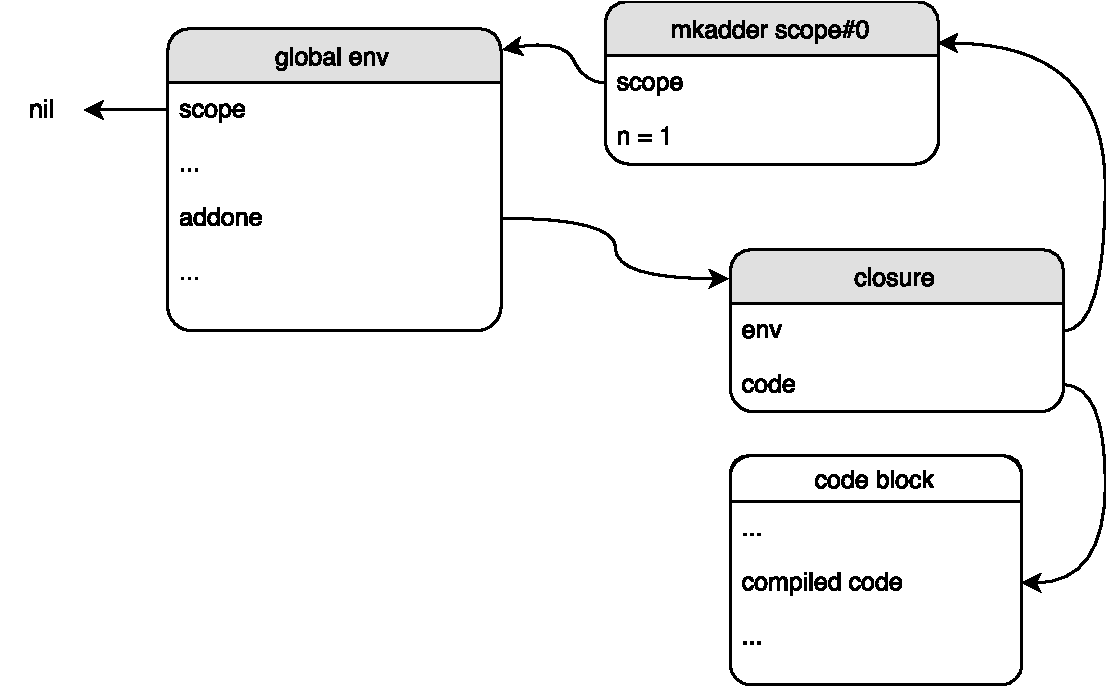
\includegraphics[width=300pt]{closure-sample.pdf}
\caption{闭包内存布局示例}
\label{fig:closure-mem-layout}
\end{figure}

在本节中,主要讨论了程序运行需要的两种上下文,而这也是EdenApple的VM所要维护的核心结构,在第\ref{ch:vm impl}章中将详细地描述如何实现VM。